% !TeX spellcheck = en_US
%
%
% v 2.3  Feb 2019   Volker RW Schaa
%		# changes in the collaboration therefore updated file "jacow-collaboration.tex"
%		# all References with DOIs have their period/full stop before the DOI (after pp. or year)
%		# in the author/affiliation block all ZIP codes in square brackets removed as it was not
%         understood as optional parameter and ZIP codes had bin put in brackets
%       # References to the current IPAC are changed to "IPAC'19, Melbourne, Australia"
%       # font for "url" style changed to "newtxtt" as it is easier to distinguish "O" and "0"
%
\documentclass[letter,
               %boxit,        % check whether paper is inside correct margins
               %titlepage,    % separate title page
               %refpage       % separate references
               biblatex,     % biblatex is used
               keeplastbox,   % flushend option: not to un-indent last line in References
               %nospread,     % flushend option: do not fill with whitespace to balance columns
               %hyphens,      % allow \url to hyphenate at "-" (hyphens)
               %xetex,        % use XeLaTeX to process the file
               %luatex,       % use LuaLaTeX to process the file
               ]{jacow}
%
% ONLY FOR \footnote in table/tabular
%
\usepackage{pdfpages,multirow,ragged2e} %
\usepackage{xspace}
%
% CHANGE SEQUENCE OF GRAPHICS EXTENSION TO BE EMBEDDED
% ----------------------------------------------------
% test for XeTeX where the sequence is by default eps-> pdf, jpg, png, pdf, ...
%    and the JACoW template provides JACpic2v3.eps and JACpic2v3.jpg which
%    might generates errors, therefore PNG and JPG first
%
\makeatletter%
	\ifboolexpr{bool{xetex}}
	 {\renewcommand{\Gin@extensions}{.pdf,%
	                    .png,.jpg,.bmp,.pict,.tif,.psd,.mac,.sga,.tga,.gif,%
	                    .eps,.ps,%
	                    }}{}
\makeatother

% CHECK FOR XeTeX/LuaTeX BEFORE DEFINING AN INPUT ENCODING
% --------------------------------------------------------
%   utf8  is default for XeTeX/LuaTeX
%   utf8  in LaTeX only realises a small portion of codes
%
\ifboolexpr{bool{xetex} or bool{luatex}} % test for XeTeX/LuaTeX
 {}                                      % input encoding is utf8 by default
 {\usepackage[utf8]{inputenc}}           % switch to utf8

\usepackage[USenglish]{babel}

%%   Lengths for the spaces in the title
%%   \setlength\titleblockstartskip{..}  %before title, default 3pt
%%   \setlength\titleblockmiddleskip{..} %between title + author, default 1em
%%   \setlength\titleblockendskip{..}    %afterauthor, default 1em

%----------------------------------------------------------

%\usepackage{subfig}
%\usepackage[final]{pdfpages}
%\usepackage{multirow}
%\usepackage{ragged2e}
%\usepackage{fixmath}
%\usepackage{alltt}
%\usepackage{xspace}
%\usepackage[strings]{underscore}    % to use "_" in text

%
% if BibLaTeX is used
%

\addbibresource{converter.bib}
\graphicspath{{figures/}}

\newcommand{\bmad}{\textit{Bmad}\xspace}
\newcommand{\xx}{\mathbf{\hat{x}}}
\newcommand{\yy}{\mathbf{\hat{y}}}
\newcommand{\zz}{\mathbf{\hat{z}}}
\newcommand{\rr}{\mathbf{\hat{r}}}
\newcommand{\sss}{\mathbf{s}}
\newcommand{\rrr}{\mathbf{r}}
\newcommand{\dxds}{\frac{dx}{ds}}
\newcommand{\dyds}{\frac{dy}{ds}}

%----------------------------------------------------

%----------------------------------------------------
\begin{document}

\title{Simulating a Positron Converter in Bmad}

\author{Authors, Cornell University, Ithaca, NY, 14850, USA}

\maketitle

%----------------------------------------------------
\begin{abstract}
A model to describe the output particle distribution generated by particles of a different species
impinging on a planar target has been developed. In particular, this model was developed to simulate
positron production in the Cornell CESR Linac.

To model a specific converter target, the output particle distribution is first sampled by tracking
particles through the converter using the Geant4 toolkit which models the fundamental physics of the
conversion process. The Monte Carlo distribution from Geant4 is fitted to a set of functions and the
function coefficients are saved for use in further simulations. The idea is that using the fit
functions in a simulation is not only more portable but is orders of magnitude faster than running
Geant4.

The output position, angular orientation, and momentum distribution is modeled. Preliminary support
for modeling the polarization distribution is also discussed.
\end{abstract}

%----------------------------------------------------
\section{Introduction}

%TODO: add references

Electron-positron accelerators require a source of positrons.
The standard method of obtaining positrons for use in an accelerator is through the use of a positron converter.
This is typically a slab of heavy metal, such as tungsten, located in a Linac.
The converter is bombarded with electrons with energies of order $\sim 100$ MeV and
the electrons emit photons via bremsstrahlung, which in turn decay to $e^+ e^-$ pairs via the reaction
\begin{align*}
e^- + Z \rightarrow e^- + Z + \gamma \rightarrow e^- + Z + e^- + e^+.
\end{align*}
At the output, non-converted electrons are then quickly filtered off with a %TODO: what kind of?
magnet, effectively "converting" a beam of incoming electrons into a beam of outgoing positrons.

While there has been some discussion in the literature regarding the bremsstrahlung energy spectrum in various materials, %TODO: cite
as well as the energy spectra of the $e^+ e^-$ secondaries, %TODO: cite
no solution that describes the kinematics of the emitted $e^+$ in terms of the kinematics of the incoming $e^-$ and the physical properties of the converter has yet been developed.

REVIEW OF THE STATE OF CONVERTER MODELING IN THE LITERATURE GOES HERE.
Previous attempts have been made at developing numerical models of a positron converter. %TODO: cite Fromowitz
However, these results have been highly specialized, and have been completely standalone solutions. 
%TODO: elaborate. What does ``standalone'' mean?
There has also been a recent demand for modeling the transfer of spin from the incoming beam of electrons to the outgoing beam of positrons. %TODO: add citation

In response, the authors have developed a positron converter model for use with the \bmad\cite{b:bmad} accelerator toolkit.
Our model is designed to be as flexible as possible, accommodating any converter material and thickness.
The model can even be extended to support other kinds of incoming and outgoing particles, and is not limited to taking electrons in and sending positrons out.
The model is also fast to use with the expensive physics calculations performed only once as the converter model is being developed. This is especially important when designing a machine with a converter as optimization simulations are typically time intensive.

%----------------------------------------------------
\section{The Converter Model}

The physical processes that occur in the positron converter to produce the bremsstrahlung photons and subsequent positrons are governed by quantum electrodynamics. %TODO: maybe add a reference?
The details of these interactions are not critical when only the aggregate behavior of the converter is of interest.
Therefore, the converter's behavior is modeled with a probability distribution, which describes the overall distribution of the produced positrons in terms of the target and incoming electron's properties. REWORD OR TAKE THIS PARAGRAPH OUT.

\subsection{Coordinate System}

For concreteness, it will be assumed that the impinging beam is composed of electrons and the
outgoing beam composed of positrons. The model itself is species agnostic.

Consider an electron incident on the upstream face of a positron converter of thickness $T$, with
momentum $p_-$ perpendicular to the face of the converter as depicted in Figure \ref{fig:coords1}.
Positrons produced in the converter emerge from the downstream face with some radial displacement
$r$ and at an angle $\theta$ relative to the horizontal, as depicted in Figure \ref{fig:coords2}.
Define the (\xx, \yy, \sss)$ coordinate system so that $\xx$ is in the direction of $\rrr$, and
$(\xx, \yy, \sss)$ is a right-handed coordinate system.

By symmetry, $\theta$ must be uniformly distributed from 0 to $2\pi$.
Therefore, the kinematic properties of the produced positrons which must be modeled are its radial displacement and outgoing momentum.
The outgoing momentum $\mathbf{p}_+ \, c$ is described in terms of its magnitude, $p_+ \, c$, and its slopes along the $\xx$ and $\yy$ directions:
\begin{align}
\frac{dx}{ds} & = \frac{p_x}{p_s} \\
\frac{dy}{ds} & = \frac{p_y}{p_s}.
\end{align}


%TODO: match figure font to document font
\begin{figure}
\centering
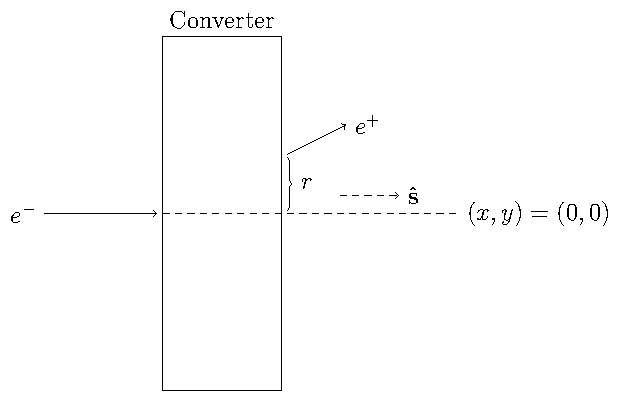
\includegraphics[width=0.45\textwidth]{coords1.pdf}
\caption{Positron converter coordinate system (side view).}
\label{fig:coords1}
\end{figure}

%TODO: make the bounding box on this figure smaller
\begin{figure}
\centering
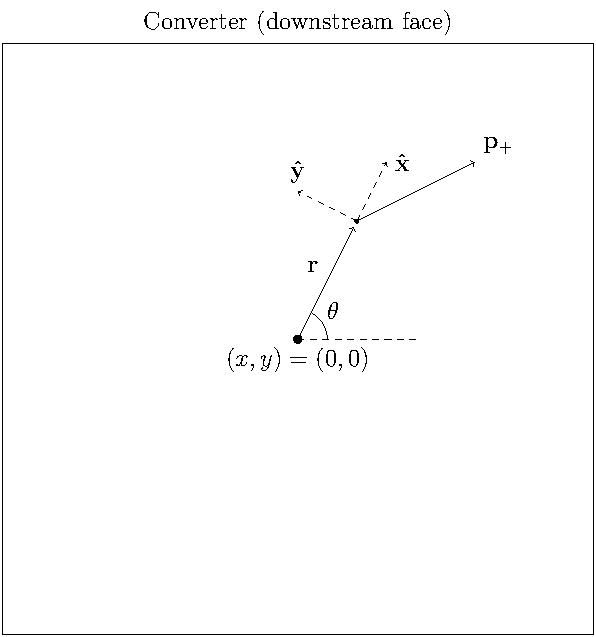
\includegraphics[width=0.4\textwidth]{coords2.pdf}
\caption{Positron converter coordinate system (view of the downstream face).}
\label{fig:coords2}
\end{figure}

\subsection{Probability Distributions}

Positrons produced in the converter are described by the distribution
\begin{align}
P \left( p_+ c, r, \dxds, \dyds \right)
\end{align}
which indicates the probability that an outgoing positron will have a given momentum and radial displacement.
$P$ is normalized to account for the efficiency of positron production:
\begin{align}
\int P \left( p_+ c, r, \dxds, \dyds \right) \, d(p_+ c) \, dr \, d \! \left( \dxds \right) d \! \left( \dyds \right) & = \frac{N_+}{N_-},
\end{align}
where $N_+$ is the total number of positrons produced, and $N_-$ is the number of electrons incident upon the converter.
To make the problem easier to grapple with, $P$ is decomposed into two subdistributions,
\begin{align}
P \left( p_+ c, r, \dxds, \dyds \right) & = P_1 \left( p_+ c, r \right) P_2 \left( \dxds, \dyds ; p_+ c, r \right)
\end{align}
which are normalized to $N_+/N_-$ and $1$ respectively.
Note that $P_2$ depends on $p_+ c$ and $r$, so that the shape of $P_2$ varies with $p_+ c$ and $r$.

Using Geant\cite{geant}, a large number of electrons incident upon the converter are simulated, and the produced positrons and their kinematics are recorded.
The produced positrons are binned into a two-dimensional histogram by their $p_+ c$ and $r$ values.
This histogram gives an approximation of $P_1$.
For $P_2$, fits are performed to $\dxds$ and $\dyds$ for the positrons in each $(p_+c, r)$ bin.
These fits yield $P_2 \left( \dxds, \dyds ; p_+ c, r \right)$.
Examples of the $P_1$ and $P_2$ distributions obtained from the Geant simulation are shown in Figures \ref{fig:p1} and \ref{fig:p2} respectively.

\begin{figure}
\centering
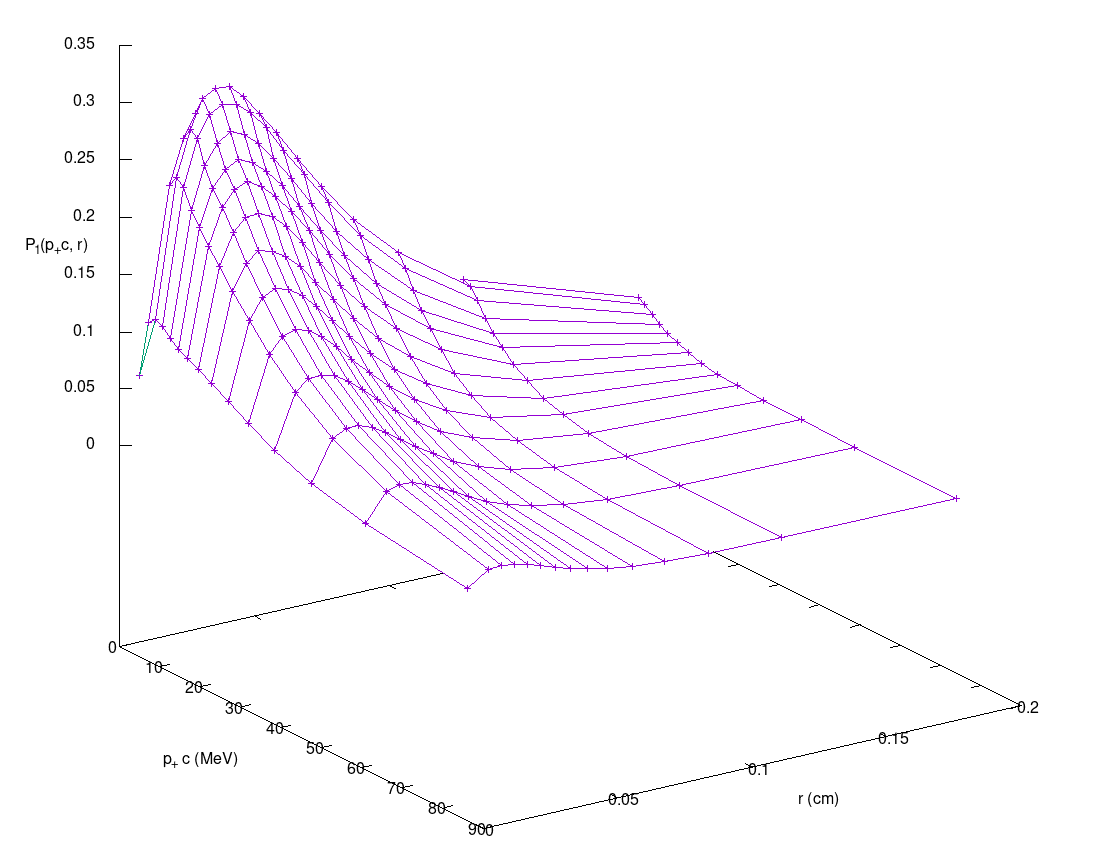
\includegraphics[width=0.45\textwidth]{p1}
\caption{$P_1(p_+ c, r)$ for incoming electrons with $p_- c = 300$ MeV and a tungsten target of thickness $T = 6.35$ mm.}
\label{fig:p1}
\end{figure}

\begin{figure}
\centering
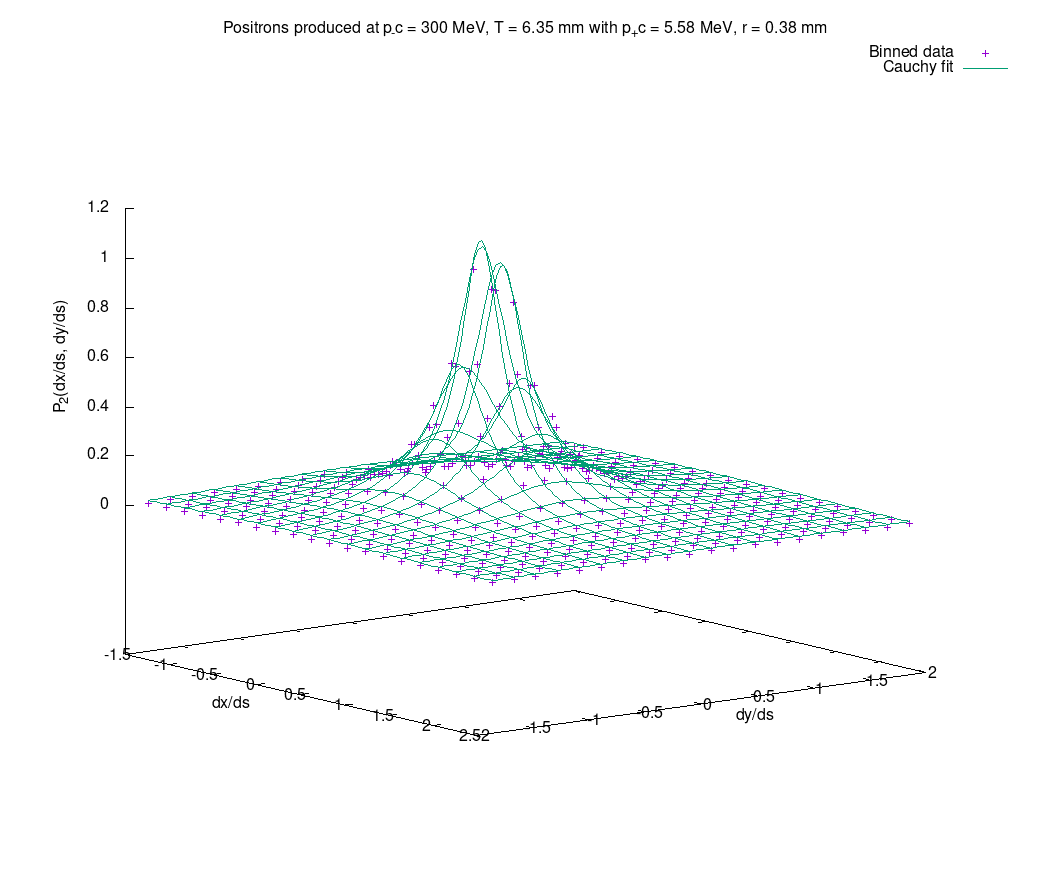
\includegraphics[width=0.45\textwidth]{p2}
\caption{$P_2 \left( \dxds, \dyds ; p_+ c, r \right)$ for incoming electrons with $p_- c = 300$ MeV and a tungsten target of thickness $T = 6.35$ mm,
and outgoing positrons with $p_+ c = 5.58$ MeV and $r = 0.38$ mm.
The purple points indicate data obtained directly from the Geant simulation, while the green curve shows the fit to the data.
}
\label{fig:p2}
\end{figure}

%\begin{itemize}
%\item
%Paraphrase and condense what is written in the documentation
%
%\end{itemize}

DISCUSS THE SITUATION IF THE INCOMING PARTICLE IS NOT PERPENDICULAR TO THE TARGET.


\section{Spin Tracking}

Polarization transfer from the incoming electrons to the outgoing positrons has also been modeled.
Any incoming polarization $\mathbf{S}_-$ may be specified, and histograms describing $S_x$, $S_y$, and $S_z$ of the produced positrons as functions of $p_+ c$ and $r$ are produced.
The authors have found that only the longitudinal polarization of the incoming electrons is ever transferred to the produced positrons; the produced positrons always have $S_x$ and $S_y$ essentially zero regardless of the incoming electron polarization.
As an example, Figure \ref{fig:sz} illustrates $S_z$ as a function of $p_+ c$ and $r$ for incoming electron with momentum $p_- c = 300$ MeV.

\begin{figure}
\centering
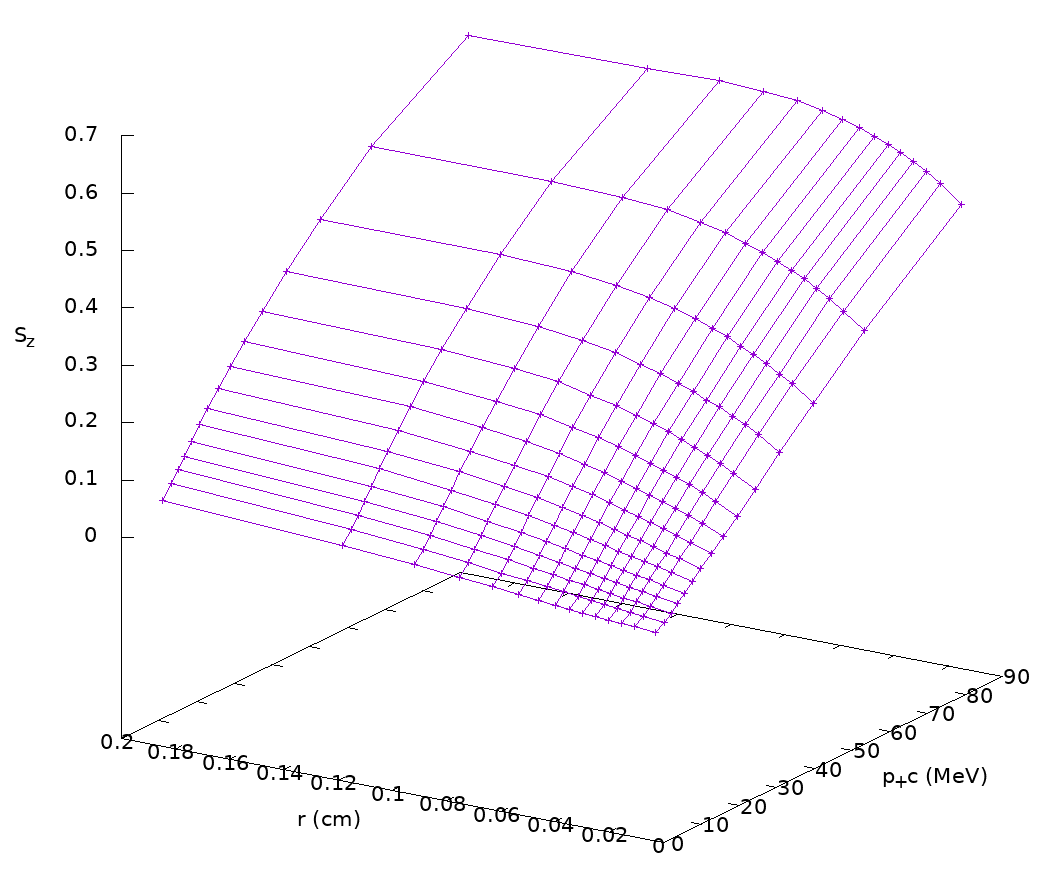
\includegraphics[width=0.45\textwidth]{sz}
\caption{Positron $S_z$ as a function of $p_+ c$ and $r$ for incoming electrons with $p_- c = 300$ MeV and a tungsten target of thickness $T = 6.35$ mm.}
\label{fig:sz}
\end{figure}

Recently, the PEPPo collaboration %TODO: cite arXiv:1606.08877
has published experimental results of polarized positron production from a polarized electron beam via bremsstrahlung, to which the spin tracking results from this simulation can be compared.
This simulation yields polarization transfer efficiencies significantly higher than those observed experimentally for outgoing positrons with $p_+ c$ less than 5 MeV.
In contrast, the simulation's results for higher momentum positrons agrees closely with experiment.
The discrepancy is likely due to approximations made by the Geant library in computing polarization transfer during the pair production step. % According to email with Eric Voutier in August 2020, reproduced below
While this disagreement shows that the spin tracking components of this simulation should not be relied on for accuracy at present, all of the infrastructure is in place to handle spin tracking.
When more accurate spin tracking methods become available in Geant, this simulation, and the \bmad \, converter element, will be ready to use their results.
%% Dear Dr. Mastroberti,
%%
%%  From the description you are giving, I would primarily question the physics you are taking into account in
%%  GEANT4 simulations. Have a look at the previous work of Jonathan Dumas in his thesis
%%
%%  https://tel.archives-ouvertes.fr/tel-00647307
%%
%%  The main point is that Olsen & Maximon calculations implemented in GEANT4 dont work for pair creation, especially
%%  in the low energy part of the positron spectra. The origin of this was tracked down to electron mass effects which
%%  persist even at high initial beam energies. This was corrected in the work below
%%
%%  arXiv:0907.5271  [pdf, ps, other]  hep-ph doi 10.1103/PhysRevC.81.055208
%%
%%  You have a short explanation of that also in
%%
%%  https://arxiv.org/pdf/1711.09659.pdf
%%
%%  So if you are using GEANT4 with Olsen & Maximon calculations, I think the disagreement is normal.
%%
%%  Hope this will help. Regards, Eric
%%
%% ----- Mail original -----
%% De: "John Mastroberti" <jmm699@cornell.edu>
%% À: "ERIC VOUTIER" <voutier@ipno.in2p3.fr>
%% Cc: "david sagan" <david.sagan@cornell.edu>, shanks@cornell.edu
%% Envoyé: Samedi 15 Août 2020 19:52:04
%% Objet: Positron Converter Polarization Simulation
%%
%% Dr. Voutier,
%%
%% Hi, my name is John Mastroberti.
%% I am a researcher at Cornell University.
%% I am working with David Sagan and Jim Shanks (CC'd) on a positron converter model based on Geant4.
%% We have recently implemented polarization tracking in our model, and we wanted to compare our model results to the results of your 2016 PRL, "Production of Highly Polarized Positrons Using Electrons at MeV Energies."
%%
%% We ran a simulation with incoming electrons of momentum 8.19 MeV with longitudinal polarization, and examined the outgoing positron polarization for positrons of momenta 3.07 MeV, 4.02 MeV, 5.34 MeV, and 6.25 MeV, as you did in your experiment.
%% We found polarization transfer efficiencies about 1.9 sigma and 2.8 sigma larger than your group did at the outgoing momenta of 3.07 MeV and 4.02 MeV respectively.
%% In contrast, our results at 5.34 MeV and 6.25 MeV agree quite closely with yours.
%% Our simulation records the polarization of the outgoing positrons directly after they emerge from the downstream face of the converter, whereas your measurement was taken after some additional beam optics.
%% Do you think this difference could account for the large discrepancy between our results and yours at the lower momenta?
%%
%% We were also wondering what physics list you used in the Geant simulations that you performed.
%% Ours is a custom list which basically just turns on all of the polarized E&M physics processes that Geant supports.
%% This may also be a cause of the discrepancy.
%%
%% Thank you,
%% John Mastroberti

% \begin{itemize}
% \item
% Discuss 2016 PRL (arXiv:1606.08877)
%
% \item
% Compare our simulation output to their experimental results
%
% \end{itemize}


%\begin{itemize}
%\item
%Give general description of how spin is recorded from the simulation
%
%\item
%Discuss results/planned experimental verification?
%
%\end{itemize}


%----------------------------------------------------
\section{The Bmad Converter Element}

The converter simulation and fitting programs aggregate their results into a single output file.
This output file provides \bmad \, with all of the binned data and fit parameters necessary to emulate the behavior of the converter.

A converter element has been added to \bmad \, which uses the model developed here to simulate a positron converter.
Previously, \bmad \, lattices could be constructed to model the elements upstream or downstream of a converter.
Now, the converter element can be used to connect these lattices together, allowing for the simulation of an entire linac end-to-end.

Since the converter simulation program samples a discrete set of incoming electron energies and target thickness, \bmad \, performs interpolation to determine the correct behavior of the converter for intermediate values.
For each incoming electron, \bmad \, randomly pulls values of $p_+ c$, $r$, $\dxds$, and $\dyds$ from the interpolated probability distributions.
The likelihood of producing a positron from the incoming electron is encoded in the weighting of the outgoing particle, a system which \bmad \, uses counting fractions of particles.

Agreement between direct output from Geant4 and emulated output from \bmad \, is quite good, with the distribution of particles from \bmad \, coming within a few percent of the Geant distributions.
This is illustrated in Figure \ref{fig:bmad}. %TODO: make hard comparisons between bmad and geant
This close agreement indicates that little accuracy is sacrificed in using the aggregate model of the converter.
Moreover, \bmad \, simulates the positron converter approximately Y times faster than the direct Geant4 physics simulations. % TODO: run timing comparisons

\begin{figure}
\centering
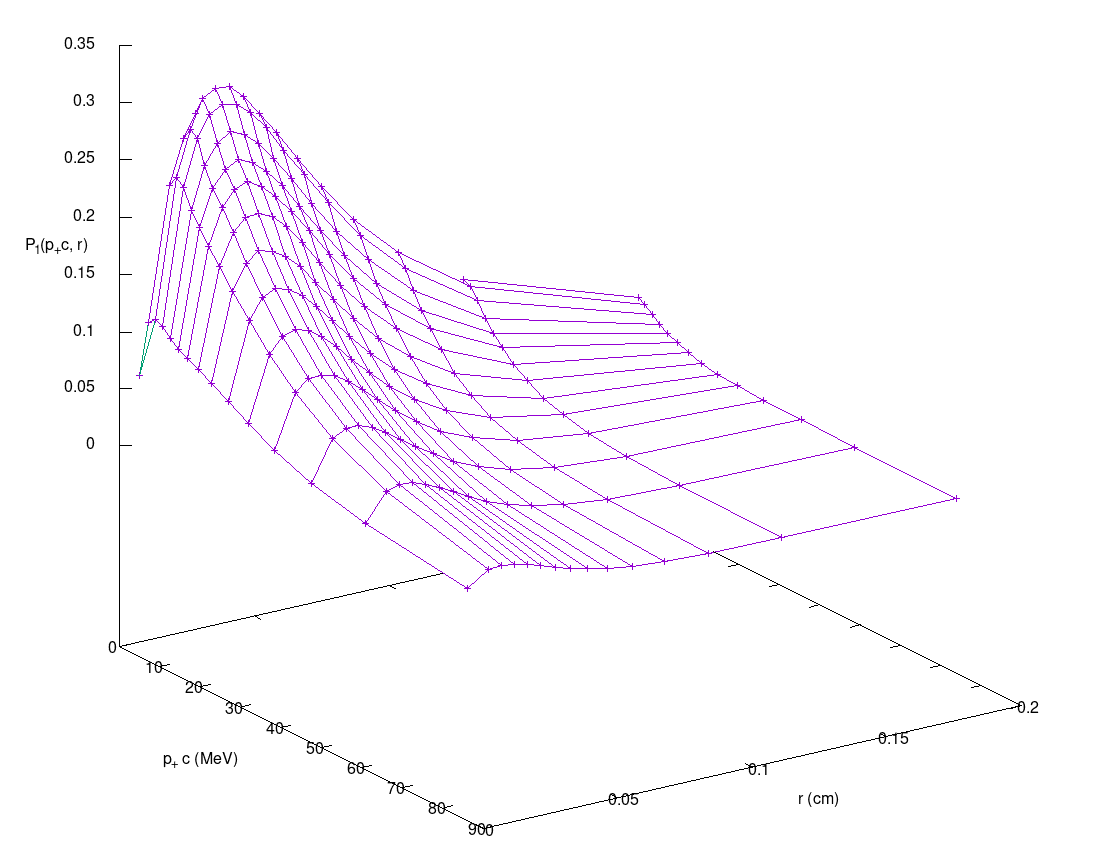
\includegraphics[width=0.45\textwidth]{p1}
\caption{Placeholder figure for comparison between Geant and Bmad.}
\label{fig:bmad}
\end{figure}

% \begin{itemize}
% \item
% Describe how simulation output is read into Bmad
%
% \item
% Discuss Bmad's scheme for generating positrons from simulation output
%
% \item
% Compare Bmad/Geant distributiions?
%
% \end{itemize}


%----------------------------------------------------
%\section{Applications}
%
%\begin{itemize}
%\item
%CESR Linac lattice
%
%\item
%Optimizations could include
%\begin{itemize}
%\item
%Tuning quad/solenoid strengths
%
%\item
%Tuning element positions
%
%\end{itemize}
%
%\item
%Discuss increase in yield due to optimizations that were made possible by the converter element?
%
%\end{itemize}


%----------------------------------------------------
\section{Conclusion}

This method of modeling the positron converter provides simulation results that are in close agreement to Geant4's direct simulation of bremsstrahlung radiation and pair production.
A small sacrifice in accuracy is made in return for a significant increase in simulation speed, making this method appropriate for use in lattice simulation and optimization software such as \bmad.

One of the primary motivators for this work was the desire to fully model the CESR linac lattice.
Work is currently underway to do so using the model developed here.
A first goal in this endeavor is to assess the agreement between the \bmad\,  model of the linac as a whole the linac's experimentally observed beam.
Once good agreement is established, \bmad \, and Tao can be used to optimize the lattice design, including quadrupole and solenoid tuning.
Other future applications could include the optimization of element positioning on the linac beam line.



%--------------------------------------------------------------------------------------
\section{Acknowledgments}

Many thanks to Vardan Khachatryan for getting us up and running with Geant.
% and any other help relevant to obtaining linac lattice,
% funding etc

%--------------------------------------------------------------------------------------

\printbibliography

\clearpage

\end{document}

